\documentclass{classrep}
\usepackage[utf8]{inputenc}


\studycycle{Informatyka, studia dzienne, inż I st.}
\coursesemester{V}
\coursename{Obliczenia naukowe}
\courseyear{2017/2018}
\courseteacher{dr hab. Paweł Zieliński}
\coursegroup{czwartek TN, 11:15}

\author{
  \studentinfo{Agata Jasionowska}{229726}
}

\title{Laboratorium \ppauza Lista 3}
\begin{document}

\maketitle

\section{Zadanie 1}
	\subsection{Opis problemu}
		Implementacja funkcji rozwiązującej równanie $f(x)=0$ metodą bisekcji.
	
	\subsection{Opis rozwiązania}
		Przebieg tej metody następuje zgodnie z widocznym Algorytmem \ref{algo:1}.
	
		\begin{algorithm}[!htbp]
    			\SetKwInOut{Input}{Input}
    			\SetKwInOut{Output}{Output}
    			
    			\SetKwProg{F}{Function}{}{}
    			\SetKwFunction{Sgn}{sgn}
    			\SetKwFunction{Mb}{mbisekcji}
    			\SetKwFunction{Fx}{f}
    			
    			\SetKwData{Eps}{$\epsilon$}    	
    			\SetKwData{Delta}{$\delta$} 		
    			\SetKwData{A}{a} 
    			\SetKwData{B}{b} 
    			
    			\SetKwData{R}{r}
			\SetKwData{V}{v}
			\SetKwData{Valuer}{v}
			\SetKwData{Valuea}{fa}
			\SetKwData{Valueb}{fb}
			\SetKwData{Err}{err}
			\SetKwData{It}{it}
			\SetKwData{Middle}{e}
			
			
			\Input{(\Fx, \A, \B, \Delta, \Eps), gdzie: \\
					\begin{tabular}{rcl}
    						{\Fx} &---& funkcja $f(x)$ zadana jako anonimowa funkcja,\\
    						{\A, \B} &---& końce przedziału początkowego,\\
    						{\Delta, \Eps} &---& dokładność obliczeń
					\end{tabular}
		    			}
		    \Output{
		    			(\R, \V, \It, \Err), gdzie: \\
		    			\begin{tabular}{rcl}
			    			{\R} & {---} & przybliżenie pierwiastka równania $f(x) = 0$,\\
			    			{\V} & {---} &  wartość $f(\R)$,\\
			    			{\It} & {---} & liczba wykonanych iteracji,\\
			    			{\Err} & {---} & sygnalizacja błędu: \\
			    				&&	     $0$ --- brak błędu, \\
					    		&&		$1$ --- funkcja nie zmienia znaku w przedziale $[\A,\B]$.    			
					\end{tabular}
		    	}
		    	
    			\F{\Mb{\A, \B, \Delta, \Eps}} {
		    
		    \R $\leftarrow 0$\;
		    \Valuer $\leftarrow 0$\;
		    	\Valuea $\leftarrow$ \Fx{\A}\;
		    	\Valueb $\leftarrow$ \Fx{\B}\;
		    	\Middle $\leftarrow \B - \A$\;
		    	\It $\leftarrow 0$\;
		    \If{$\Sgn(\Valuea) = \Sgn(\Valueb)$} {
		    		\KwRet (\R, \Valuer, \It, 1) \;
		    	}
		    	\While{\Middle $>$ \Eps} {
		    		\It $\leftarrow \It + 1$\;
    				\Middle $\leftarrow \Middle / 2$\;
    				\R $\leftarrow$ \A + \Middle\;
    				\Valuer $\leftarrow$ \Fx{\R}\;
    				\If{$|\Middle| < \Delta \lor |\Valuer| < \Eps$} {
    					\KwRet (\R, \Valuer, \It, 0)\;
    				}
    				\eIf{$\Sgn(\Valuer) \neq \Sgn(\Valuea)$} {
    					\B $\leftarrow$ \R\;
    					\Valueb $\leftarrow$ \Valuer\;
    				}
    				{
    				\A $\leftarrow$ \R\;
    				\Valuea $\leftarrow$ \Valuer\;
    				}
    			}
    			\KwRet (\R, \Valuer, \It, 0)\;
    			}
    			\caption{Metoda bisekcji}
    			\label{algo:1}
		\end{algorithm}	
		
		Niektóre elementy pseudokodu warto uzupełnić dodatkowym komentarzem. Jako pierwszym ze spostrzeżeń można uczynić sposób obliczania punktu środkowego, czyli instrukcję: $r \leftarrow a+(b-a)/2$. Okazuje się, że w obliczeniach numerycznych o wiele lepszym rozwiązaniem jest obliczanie nowej wielkości poprzez niewielką poprawkę poprzedniej. Dlatego też wyżej wspomniane przypisanie nie ma postaci: $r \leftarrow (a+b)/2$. W pewnych przypadkach zastosowanie takiej konstrukcji mogłoby prowadzić do uzyskania wartości znajdującej się nawet poza przedziałem $[a,b]$.
		Drugą sprawą będzie sposób badania zmiany znaku wartości funkcji. Otóż wykorzystanie nierówności $fa\cdot fb < 0$ może prowadzić do nadmiaru lub niedomiaru spowodowanego mnożeniem. Zamiast tego skorzystano z $\texttt{sgn}(fa) \neq \texttt{sgn}(fb)$, unikając w ten sposób zbędnego działania.
		Ostatnim spostrzeżeniem będzie zwrócenie uwagi na warunki zakończenia obliczeń przez funkcję. Uwzględnia ona warunek $e > \epsilon$ (czy w zadanym przedziale możliwa jest kolejna iteracja), $|e| < \delta$ (gdy uzyskano już wystarczająco mały błąd) oraz $|v| < \epsilon$ (wartość funkcji w punkcie jest dostatecznie bliska zeru). Rozpatrywanie aż trzech kryteriów zakończenia pracy daje algorytmowi pewność w działaniu nawet dla przypadków patologicznych.
	
\section{Zadanie 2}
	\subsection{Opis problemu}
		Implementacja funkcji rozwiązującej równanie $f(x)=0$ metodą stycznych (Newtona).
		
	\subsection{Opis rozwiązania}	
		Działanie metody jest zgodnie z Algorytmem \ref{algo:2}.
	
		\begin{algorithm}[!htbp]
			\SetKwData{R}{r}
			\SetKwData{Err}{err}
			\SetKwData{Valuer}{v}
			\SetKwData{V}{v}
			\SetKwData{It}{it}
			\SetKwData{X}{x}
			
			\SetKwProg{F}{Function}{}{}
    			\SetKwFunction{Sgn}{sgn}
    			\SetKwFunction{Mb}{mstycznych}
    			\SetKwFunction{Fx}{f}
    			\SetKwFunction{Pf}{pf}
    			
    			\SetKwData{Eps}{$\epsilon$}    	
    			\SetKwData{Delta}{$\delta$} 	
    			\SetKwData{XX}{x0}	
    			\SetKwData{Maxit}{maxit}
    			\SetKwData{A}{a} 
    			\SetKwData{B}{b}
			
    			\SetKwInOut{Input}{Input}
    			\SetKwInOut{Output}{Output}

			\Input{(\Fx, \Pf, \XX, \Delta, \Eps, \Maxit), gdzie: \\
					\begin{tabular}{rcl}
    						{\Fx, \Pf} &---& funkcja $f(x)$ oraz $f'(x)$ zadane jako anonimowe funkcje,\\
    						{\XX} &---& przybliżenie początkowe,\\
    						{\Delta, \Eps} &---& dokładność obliczeń, \\
    						{\Maxit} &---& maksymalna dopuszczalna liczba iteracji
					\end{tabular}
		    			}
		    \Output{	(\R, \V, \It, \Err), gdzie: \\
		    			\begin{tabular}{rcl}
			    			{\R} & {---} & przybliżenie pierwiastka równania $f(x) = 0$,\\
			    			{\V} & {---} &  wartość $f(\R)$,\\
			    			{\It} & {---} & liczba wykonanych iteracji,\\
			    			{\Err} & {---} & sygnalizacja błędu: \\
			    				&&	     $0$ --- metoda zbieżna, \\
					    		&&		$1$ --- nie osiągnięto wymaganej dokładności w \Maxit iteracji, \\
					    		&&		$2$ --- pochodna bliska zeru.			
					\end{tabular}
		    	}
		    	
    			\F{\Mb{\Fx, \Pf, \XX, \Delta, \Eps, \Maxit}} {
		    
		    	\R $\leftarrow$ \XX\;
		    	\Valuer $\leftarrow \Fx{\R}$\;
		    	\It $\leftarrow 0$\;
		    \If{$|\Pf{\R}| < \Eps$} {
		    		\KwRet (\R, \Valuer, \It, 2)\;
		    	}
		    	\For{\It $\gets 1$ \KwTo \Maxit} {
		    		\X $\leftarrow \R - (\Valuer / \Pf{\R})$\;
		    		\Valuer $\leftarrow \Fx{\X}$\;
		    		\If{$|\R - \X| < \Delta \lor |\Valuer| < \Eps$} {
		    			\R $\leftarrow \X$\;
		    			\KwRet (\R, \Valuer, \It, 0)\;
		    		}
		    		\R $\leftarrow$ \X\;
    			}
    			\KwRet (\R, \Valuer, \It, 1)\;
    			}
    			\caption{Metoda stycznych}
    			\label{algo:2}
		\end{algorithm}	
	
\section{Zadanie 3}
	\subsection{Opis problemu}
		Implementacja funkcji rozwiązującej równanie $f(x)=0$ metodą siecznych(Eulera).
	
	\subsection{Opis rozwiązania}		
		Przebieg tej metody następuje zgodnie z Algorytmem \ref{algo:3}.
		
		\begin{algorithm}[!htbp]
			\SetKwData{A}{a}
			\SetKwData{B}{b}
			\SetKwData{R}{r}
			\SetKwData{Err}{err}
			\SetKwData{V}{v}
			\SetKwData{Valuea}{fa}
			\SetKwData{Valueb}{fb}
			\SetKwData{It}{it}
			\SetKwData{S}{s}
    			\SetKwInOut{Input}{Input}
    			\SetKwInOut{Output}{Output}
    			
    			\SetKwProg{F}{Function}{}{}
    			\SetKwFunction{Sgn}{sgn}
    			\SetKwFunction{Swap}{swap}
    			\SetKwFunction{Mb}{msiecznych}
    			\SetKwFunction{Fx}{f}
    			\SetKwFunction{Pf}{pf}
    			
    			\SetKwData{Eps}{$\epsilon$}    	
    			\SetKwData{Delta}{$\delta$} 	
    			\SetKwData{XX}{x0}	
    			\SetKwData{XY}{x1}	
    			\SetKwData{Maxit}{maxit}
    			\SetKwData{A}{a} 
    			\SetKwData{B}{b}

			\Input{(\Fx, \XX, \XY, \Delta, \Eps, \Maxit), gdzie: \\
					\begin{tabular}{rcl}
    						{\Fx} &---& funkcja $f(x)$ zadana jako anonimowa funkcja,\\
    						{\XX, \XY} &---& przybliżenia początkowe,\\
    						{\Delta, \Eps} &---& dokładność obliczeń, \\
    						{\Maxit} &---& maksymalna dopuszczalna liczba iteracji
					\end{tabular}
		    			}
		    \Output{	(\R, \V, \It, \Err), gdzie: \\
		    			\begin{tabular}{rcl}
			    			{\R} & {---} & przybliżenie pierwiastka równania $f(x) = 0$,\\
			    			{\V} & {---} &  wartość $f(\R)$,\\
			    			{\It} & {---} & liczba wykonanych iteracji,\\
			    			{\Err} & {---} & sygnalizacja błędu: \\
			    				&&	     $0$ --- metoda zbieżna, \\
					    		&&		$1$ --- nie osiągnięto wymaganej dokładności w \Maxit iteracji.
					\end{tabular}	    			
		    	}
		    
    			\F{\Mb{\Fx, \XX, \XY, \Delta, \Eps, \Maxit}} {		    
		    
		    	\A $\leftarrow$ \XX\;
		    	\B $\leftarrow$ \XY\;
		    	\Valuea $\leftarrow$ \Fx{\A}\;
		    	\Valueb $\leftarrow$ \Fx{\B}\;
		    	\It $\leftarrow 0$\;
		    	
		    	\For{\It $\gets 1$ \KwTo \Maxit} {
		    		\If{$|\Valuea| > |\Valueb|$} {
		    			\Swap{\A, \B}\;
		    			\Swap{\Valuea, \Valueb}\;
		    		}
		    		\S $\leftarrow (\B - \A) / (\Valueb - \Valuea)$\;
		    		\B $\leftarrow \A$\;
		    		\Valueb $\leftarrow \Valuea$\;
		    		
		    		\A $\leftarrow \A - (\Valuea \cdot \S)$\;
		    		\Valuea $\leftarrow \Fx{\A}$\;		    		
		    		
    				\If{$|\Valuea| < \Eps \lor |\B - \A| < \Delta$} {
    					\KwRet (\A, \Valuea, \It, 0)\;
    				}
    			}
    			\KwRet (\A, \Valuea, \It, 1)\;
    			}
    			\caption{Metoda siecznych}
    			\label{algo:3}
		\end{algorithm}	
			
		W widocznym Algorytmie \ref{algo:3} wartym podkreślenia jest cel zastosowania funkcji \texttt{swap}. Przestawia ona końce przedziału $a$ i $b$, gdy utrzymanie $|f(a)| \leq |f(b)|$ tego wymaga. Dlatego też, począwszy od drugiego kroku, wartości bezwzględne funkcji w kolejnych punktach są nierosnące.
\section{Zadanie 4}
	\subsection{Opis problemu}
		Przy użyciu metod zaprogramowanych w poprzednich zadaniach wyznaczenie pierwiastka równania $\sin(x)-(\frac{1}{2}x)^2=0$ dla poniższych danych:
		\begin{enumerate}[1.]
			\item Metodą bisekcji z przedziałem początkowym $[1.5,2],~\delta=\frac{1}{2}10^{-5},~\epsilon=\frac{1}{2}10^{-5}$;
			\item Metodą Newtona z przybliżeniem początkowym $x_0=1.5,~\delta=\frac{1}{2}10^{-5},~\epsilon=\frac{1}{2}10^{-5}$;
			\item Metodą siecznych z przybliżeniem początkowym $x_0=1,~x_1=2,~\delta=\frac{1}{2}10^{-5},~\epsilon=\frac{1}{2}10^{-5}$.
		\end{enumerate}
		
	\subsection{Opis rozwiązania}
		Zastosowano metody utworzone w zadaniach 1-3 wraz z zaimplementowaną funkcją $f(x)=\sin(x)-(\frac{1}{2}x)^2$ oraz jej pochodną $pf(x)=\cos(x)-\frac{1}{2}x$ (niezbędną przy korzystaniu z metody stycznych).  Miejsca zerowe zadanej funkcji widoczne są na Rysunku \ref{fig:3}.
		
		\begin{figure}[!htbp]
			\centering
			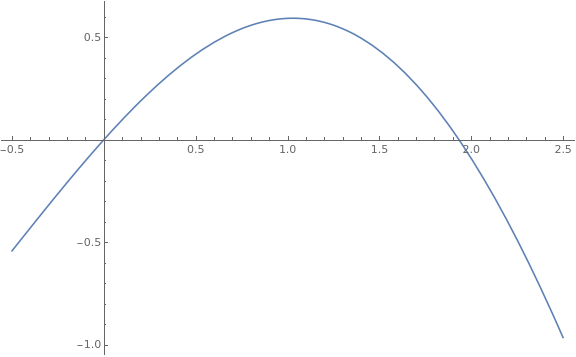
\includegraphics[width=0.8\textwidth]{zadania/plot41.png}
  			\caption{Wykres funkcji $\sin(x)-(\frac{1}{2}x)^2=0$.}
  			\label{fig:3}
		\end{figure}	
		
	
	\subsection{Wyniki}
		Uzyskane rezultaty widoczne są w Tabeli \ref{table:1}.
		
		\begin{table}[!hpbt]
        		\centering
        		\footnotesize
			\sisetup{
				table-number-alignment = right,
				table-figures-integer = 1,
				table-figures-decimal = 16,
				table-figures-exponent = 1
			}
			\begin{tabular}{lSSl} \toprule
				{podpunkt} & {$x_0$} & {$f(x_0)$} & {liczba iteracji}\\ \midrule
				$1.$ & 1.9337539672851562 & -2.7027680138402843e-7 & 16 \\ 
	 			$2.$ & 1.933753779789742 & -2.2423316314856834e-8 & 4 \\
	 			$3.$ & 1.9337509005356321 & 3.783706985283075e-6 & 4 \\ \bottomrule
	 		\end{tabular}
	 		\caption{$\sin(x)-(\frac{1}{2}x)^2=0$ dla danych z zadania.}
			\label{table:1}
		\end{table}	
		
	\subsection{Wnioski}
		Przykład funkcji podanej w tym zadaniu pokazuje różnice w liczbie iteracji wykonywanych przez każdą z trzech metod wyznaczania pierwiastków równań. Funkcja metody bisekcji wykonała ich najwięcej, bo aż 17, aby uzyskać wynik z zadaną dokładnością. O wiele lepiej radzą tu sobie funkcje siecznych oraz stycznych - wymagana precyzja została osiągnięta już po 4 przebiegach.
		Uzyskane rezultaty znajdują swoje potwierdzenie w teoretycznej zbieżności wyżej wymienionych metod. Otóż posortowanie według tego współczynnika daje w efekcie następującą kolejność metod: Newtona (kwadratowo), siecznych ($\approx 1.62$, nadliniowo) oraz bisekcji (liniowo). 
		Przeprowadzenie analizy otrzymanych w Tabeli \ref{algo:1} wyników mogłoby prowadzić do śmiałego wniosku, iż ostatnia z nich jest nie tylko najwolniejsza, ale także najmniej dokładna. Bardziej trafnym jest jednak zauważenie, że zwrócona przez metodę bisekcji wartość jest najbliższa zadanej dokładności (przez co można by nazwać ją najbardziej "stabilną" z wszystkich badanych). 
		W przypadku dwóch pozostałych --- zbiegały one szybciej, co doprowadziło finalnie do osiągnięcia większej dokładności oraz obliczenia pierwiastka najbliższego rzeczywistemu. Warto mieć na uwadze, iż wybór odmiennej funkcji bądź przedziałów skutkować może uzyskaniem zupełnie innych rezultatów.
		
%		Zauważenia wymaga fakt, iż każdy krok metody siecznych wymaga obliczenia tylko jednej wartości funkcji, zaś w metodzie Newtona trzeba obliczyć dwie takie wartości, mianowicie $f(x)$ i $f'(x)$. W obu metodach najbardziej kosztowne jest właśnie obliczanie wartości funkcji i w tym sensie para kroków metody siecznych jest porównywalna z jednym krokiem metody Newtona.
\section{Zadanie 5}
	\subsection{Opis problemu}
		Wyznaczenie przy pomocy metody bisekcji wartości zmiennej $x$, dla której następuje przecięcie wykresów funkcji $y=3x$ oraz $y=\exp(x)$ dla dokładności $\delta=10^{-4}$, $\epsilon=10^{-4}$.
	
	\subsection{Opis rozwiązania}
		W celu rozwiązania zadania zastosowano metodę \texttt{mbisekcji} utworzoną w zadaniu 1.
		Aby określić miejsce przecięcia zadanych funkcji należy znaleźć taki punkt, dla którego przyjmują one identyczną wartość dla tego samego argumentu, czyli $f(x)=3x-\exp(x)$. 	\\
		 Najprostszym sposobem określenia przedziałów początkowych będzie analiza wykresu obu funkcji. Z Rysunku \ref{fig:1} wywnioskować można, iż poszukiwane wyniki znajdą się w przedziałach $[0.0,1.0]$ oraz $[1.0,2.0]$.
		
		\begin{figure}[!htbp]
			\centering
			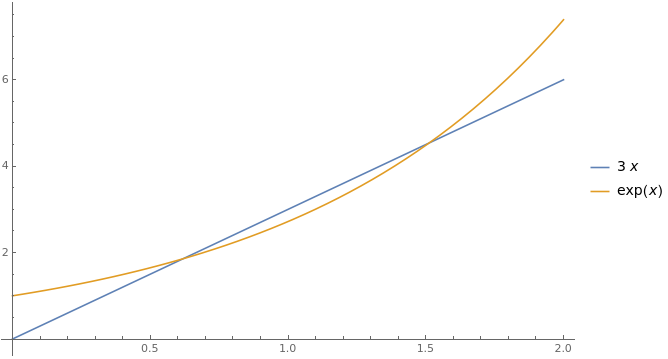
\includegraphics[width=0.8\textwidth]{zadania/plot51.png}
  			\caption{Wykres funkcji $y=3x$ oraz $y=\exp(x)$.}
  			\label{fig:1}
		\end{figure}	
		
	\subsection{Wyniki}
		Poniższa tabela prezentuje otrzymane rozwiązania:
		\begin{table}[!hpbt]
        		\centering
        		\footnotesize
			\sisetup{
				table-number-alignment = right,
				table-figures-integer = 1,
				table-figures-decimal = 12
			}
			\begin{tabular}{lSl} \toprule
				{przedział} & {$x$} & {liczba iteracji}\\ \midrule
				$[0.0,1.0]$ & 0.619140625 & $9$ \\ 
	 			$[1.0,2.0]$ & 1.5120849609375 & $13$ \\ \bottomrule
	 		\end{tabular}
	 		\caption{Miejsca zerowe $f(x)=3x-\exp(x)$ obliczone z pomocą metody bisekcji.}
			\label{table:2}
		\end{table}	
		
	\subsection{Wnioski}
		Ważnym czynnikiem wpływającym na pomyślne znalezienie pierwiastków funkcji metodą bisekcji jest umiejętny dobór przedziału początkowego. Należy zwrócić uwagę, iż w tym przypadku uruchomienie jej dla przedziału $[0.0,2.0]$ zwróci błąd związany z niezmiennością znaku. Jednak po wyszczególnieniu $[0.0,1.0]$ i $[1.0,2.0]$ znalezienie miejsc zerowych $f(x)$ nie nastręcza problemów. Pomocna w czynności wyboru startowego przedziału może być na przykład analiza wykresu funkcji, którą zastosowano w rozwiązaniu tego problemu. Zadanie okazałoby się jednak znacznie trudniejsze, gdyby takie rozwiązanie nie było dostępne. W związku ze stosunkowo niewielką długością przedziałów, niezbędna byłaby dobra znajomość przebiegu zadanej funkcji bądź przeprowadzenie wielu eksperymentów. 
		
\section{Zadanie 6}
	\subsection{Opis problemu}
		Znalezienie pierwiastków funkcji $f_1(x)=\exp(1-x)-1$ oraz $f_2(x)=x\exp(-x)$ przy pomocy metod: bisekcji, stycznych oraz siecznych z dokładnością obliczeń $\delta=10^{-4}$, $\epsilon=10^{-4}$. Należy zadbać o dobór odpowiedniego przedziału oraz przybliżeń początkowych.
		
	\subsection{Opis rozwiązania}
		W rozwiązaniu zadania zastosowano metody \texttt{mbisekcji}, \texttt{msiecznych} oraz \texttt{mstycznych}, utworzone w zadaniach 1-3.
		Rozpoczęto od przeprowadzenia analizy wykresów (Rysunek \ref{fig:2}) zadanych funkcji w celu określenia najlepszych parametrów.
		
		\begin{figure}[!htbp]
			\centering
			\subfloat[1.][$f_1(x)=\exp(1-x)-1$]{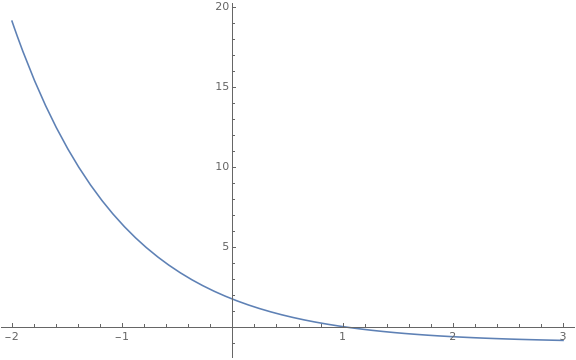
\includegraphics[width=0.5\textwidth]{zadania/plot61.png}} \hfill
			\subfloat[2.][$f_2(x)=x\exp(-x)$]{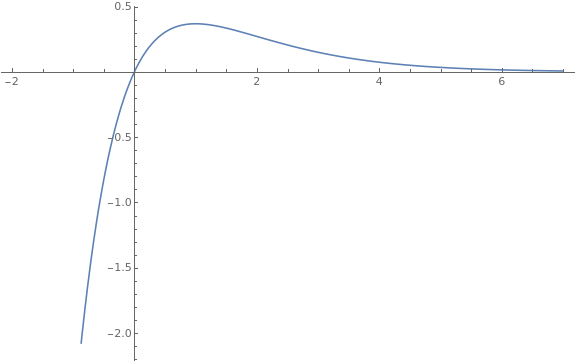
\includegraphics[width=0.5\textwidth]{zadania/plot62.png}}
  			\caption{}
  			\label{fig:2}
		\end{figure}		
		
	\subsection{Wyniki}
			Z wykresu z łatwością odczytać można prawidłowe rozwiązanie $f_1(x)=\exp(1-x)-1$, jakim jest $x=1.0$.
			Dla metody bisekcji unikano sytuacji, gdy pierwiastek znajduje się w środku przedziału początkowego. Podczas używania metody Newtona należało uważać przy dobieraniu $x_0$, gdyż pochodna dąży do $0$, co jest niepożądane dla tej metody. W funkcji metody siecznych wybranie zbyt dużych wartości przybliżeń sprawi, że obliczenia wykonane są na bliskich sobie wartościach i działanie zakończy się szybko ze względu na osiągnięcie założonej precyzji.
			\\
			
			W przypadku funkcji $f_2(x)=x\exp(-x)$ już sam jej wzór wskazuje właściwy pierwiastek, czyli $x=0.0$. Zastosowano podobne środki ostrożności co w przypadku funkcji $f_1(x)$.
		\begin{table}[!hpbt]
        		\centering
        		\footnotesize
			\sisetup{
				table-number-alignment = right,
				table-figures-integer = 2,
				table-figures-decimal = 16,
				table-figures-exponent = 2
			}
			\begin{tabular}{llSSc} \toprule
				{metoda} & {początkowe dane} &{$x$} & {$f(x)$} & {liczba iteracji}\\ \midrule
				bisekcji & $[a,b]=[0.1,1.2]$ & 0.9999938964843748 & 6.103534251789e-6 & $14$ \\ 
				bisekcji & $[a,b]=[-0.1,1.4]$ & 1.000006103515625 & -6.103496998477453e-6 & $14$ \\ 
				bisekcji & $[a,b]=[0.0,150]$ & 0.9999990463256836 & 9.536747711536009e-7 & $21$ \\
	 			stycznych & $x_0=0.3$ & 0.9999999866969493 & 1.3303050661050975e-8 & $4$ \\
	 			siecznych & $x_0=-0.4,~x_1=1.3$ & 1.0000026160714057 & -2.6160679837961e-6 & $7$ \\ 
	 			siecznych & $x_0=-2.0,~x_1=2.0$ & 1.0000063854903036 & -6.385469916381226e-6 & $23$ \\ \bottomrule
	 		\end{tabular}
	 		\caption{$f_1(x)=\exp(1-x)-1$.}
			\label{table:3}
		\end{table}
		
		\begin{table}[!hpbt]
        		\centering
        		\footnotesize
			\sisetup{
				table-number-alignment = right,
				table-figures-integer = 2,
				table-figures-decimal = 16,
				table-figures-exponent = 2
			}
			\begin{tabular}{llSSc} \toprule
				{metoda} & {początkowe dane} &{$x$} & {$f(x)$} & {liczba iteracji}\\ \midrule
				bisekcji & $[a,b]=[-0.4,0.7]$ & -4.5776367187399074e-6 & -4.577657673545798e-6 & 16 \\ 
	 			stycznych & $x_0=0.4$ & -8.878980981560664e-6 & -8.879059818213929e-6 & 4 \\  	
	 			siecznych & $x_0=-1.0,~x_1=0.3$ & 9.44134425373555e-6 & 9.441255115175028e-6 & 23 \\
	 			siecznych & $x_0=-0.1,~x_1=0.9$ & 1.10233618098865e-6 & 1.102334965844264e-6 & 6 \\ \bottomrule
	 		\end{tabular}
	 		\caption{$f_2(x)=x\exp(-x)$.}
			\label{table:4}			
		\end{table}	

		\begin{table}[!hpbt]
        		\centering
        		\footnotesize
			\sisetup{
				table-number-alignment = right,
				table-figures-integer = 1,
				table-figures-decimal = 16,
				table-figures-exponent = 1
			}
			\begin{tabular}{lSScc} \toprule
				{$x_0$} & {$x$} & {$f(x)$} & {liczba iteracji} & {błąd} \\ \midrule
				\multicolumn{4}{c}{$f_1$} \\ \hline
				$1.5$ & 0.9999999984736215 & 1.5263785790864404e-9 & $4$ & 0\\ 
				$2.5$ & 0.9999934982589662 & 6.501762170207925e-6 & $6$ & 0\\
	 			$5.5$ & 0.9999998543788339 & 1.4562117667260566e-7 & $89$ & 0\\
	 			$7.5$ & {---} & {---} & {---} & 1\\
	 			$13$ & {---} & {---} & {---} & 2\\ \hline
	 			\multicolumn{4}{c}{$f_2$} \\ \hline
	 			$1.0$ & {---} & {---} & {---} & 2 \\ 
	 			$2.0$ & 14.398662765680003 & 8.036415344217211e-6 & $10$ & 0\\ 
	 			$5.0$ & 15.194283983439147 & 3.827247505782993e-6 & $9$ & 0\\
	 			$10.0$ & 14.380524159896261 & 8.173205649825554e-6 & $4$ & 0\\ 
	 			$50.0$ & 50.0 & 9.643749239819589e-21 & $0$ & 2\\ \bottomrule
	 		\end{tabular}
	 		\caption{Metoda Newtona dla $f_1(x)=\exp(1-x)-1$ oraz $f_2(x)=x\exp(-x)$.}
			\label{table:5}			
		\end{table}	

	\subsection{Wnioski}
		Zestawienie wyników z Tabel \ref{table:3} oraz \ref{table:4} widocznych powyżej pozwala na wyciągnięcie kilku wniosków. Otóż metoda bisekcji nie ma żadnych ograniczeń związanych z przebiegiem zadanej funkcji oraz jej pochodnej (w przeciwieństwie np. do metody Newtona). Niezależnie od przesunięć przedziału względem poprawnego pierwiastka wylicza wynik w tym samym tempie zależnym od wielkości przedziału (ma to sens, gdyż metoda ta polega na sukcesywnym dzieleniu przedziału na pół aż do momentu uzyskania takiego o satysfakcjonująco małym rozmiarze). Metoda stycznych najlepiej radzi sobie z wyznaczaniem pierwiastka, gdy kluczem jest szybkość --- ze wszystkich badanych metod zwracała ona rozwiązanie po najmniejszej liczbie wykonanych iteracji. Nie oznacza to jednak, że jest najlepszym wyborem w każdej sytuacji --- należy brać pod uwagę jej ograniczenia, nakładane przez konieczność obliczania pochodnej funkcji.  \\
	
		Zadanie 
		TEMP NOTES:	 \\
		Wnioski dla wyników metody Newtona przy szczególnych argumentach!!!		
		Dla pierwszego: nie udało się wyliczyć dla $x_0=8$ - wciąż niewystarczająca była obrana liczba iteracji wynosząca $it=10000000000$.
		Dla drugiego: podanie argumentu początkowego $x_0=1.0$ powodowało zwrócenie błędu --- pochodna bliska wartości $0.0$.
		
\end{document}
